\documentclass[aspectratio=169]{beamer}
\usepackage[T1]{fontenc}
\usepackage[utf8]{inputenc}
\usepackage{listings}
\usepackage{colortbl}
\usepackage[scaled=.92]{helvet}
\renewcommand*\sfdefault{cmss}
\usepackage[sfmath]{kpfonts}

\definecolor{codegreen}{rgb}{0,0.6,0}
\definecolor{codegray}{rgb}{0.5,0.5,0.5}
\definecolor{codepurple}{rgb}{0.58,0,0.82}
\definecolor{backcolour}{rgb}{0.95,0.95,0.92}

\title{Kowalski - Your Helpful \\AI Assistant}
\author{Christian Goll <\texttt{cgoll@suse.com}>}
\date{\today}
\usetheme{suse}

\begin{document}
\begin{frame}
  \titlepage
\end{frame}

\begin{frame}{Outline}
  \tableofcontents
\end{frame}

\section{Introduction}
\begin{frame}[fragile]{The Challenge: LLMs and System Configuration}
\begin{columns}
\column{0.5\textwidth}
  \begin{block}{Current state}
    \begin{itemize}
      \item Large Language Models (LLMs) are powerful for general tasks.
      \item LLMs are allready used for system configuration tasks
      \item Halucinations and wrong tools likely to be presented
    \end{itemize}
  \end{block}
\column{0.5\textwidth}
  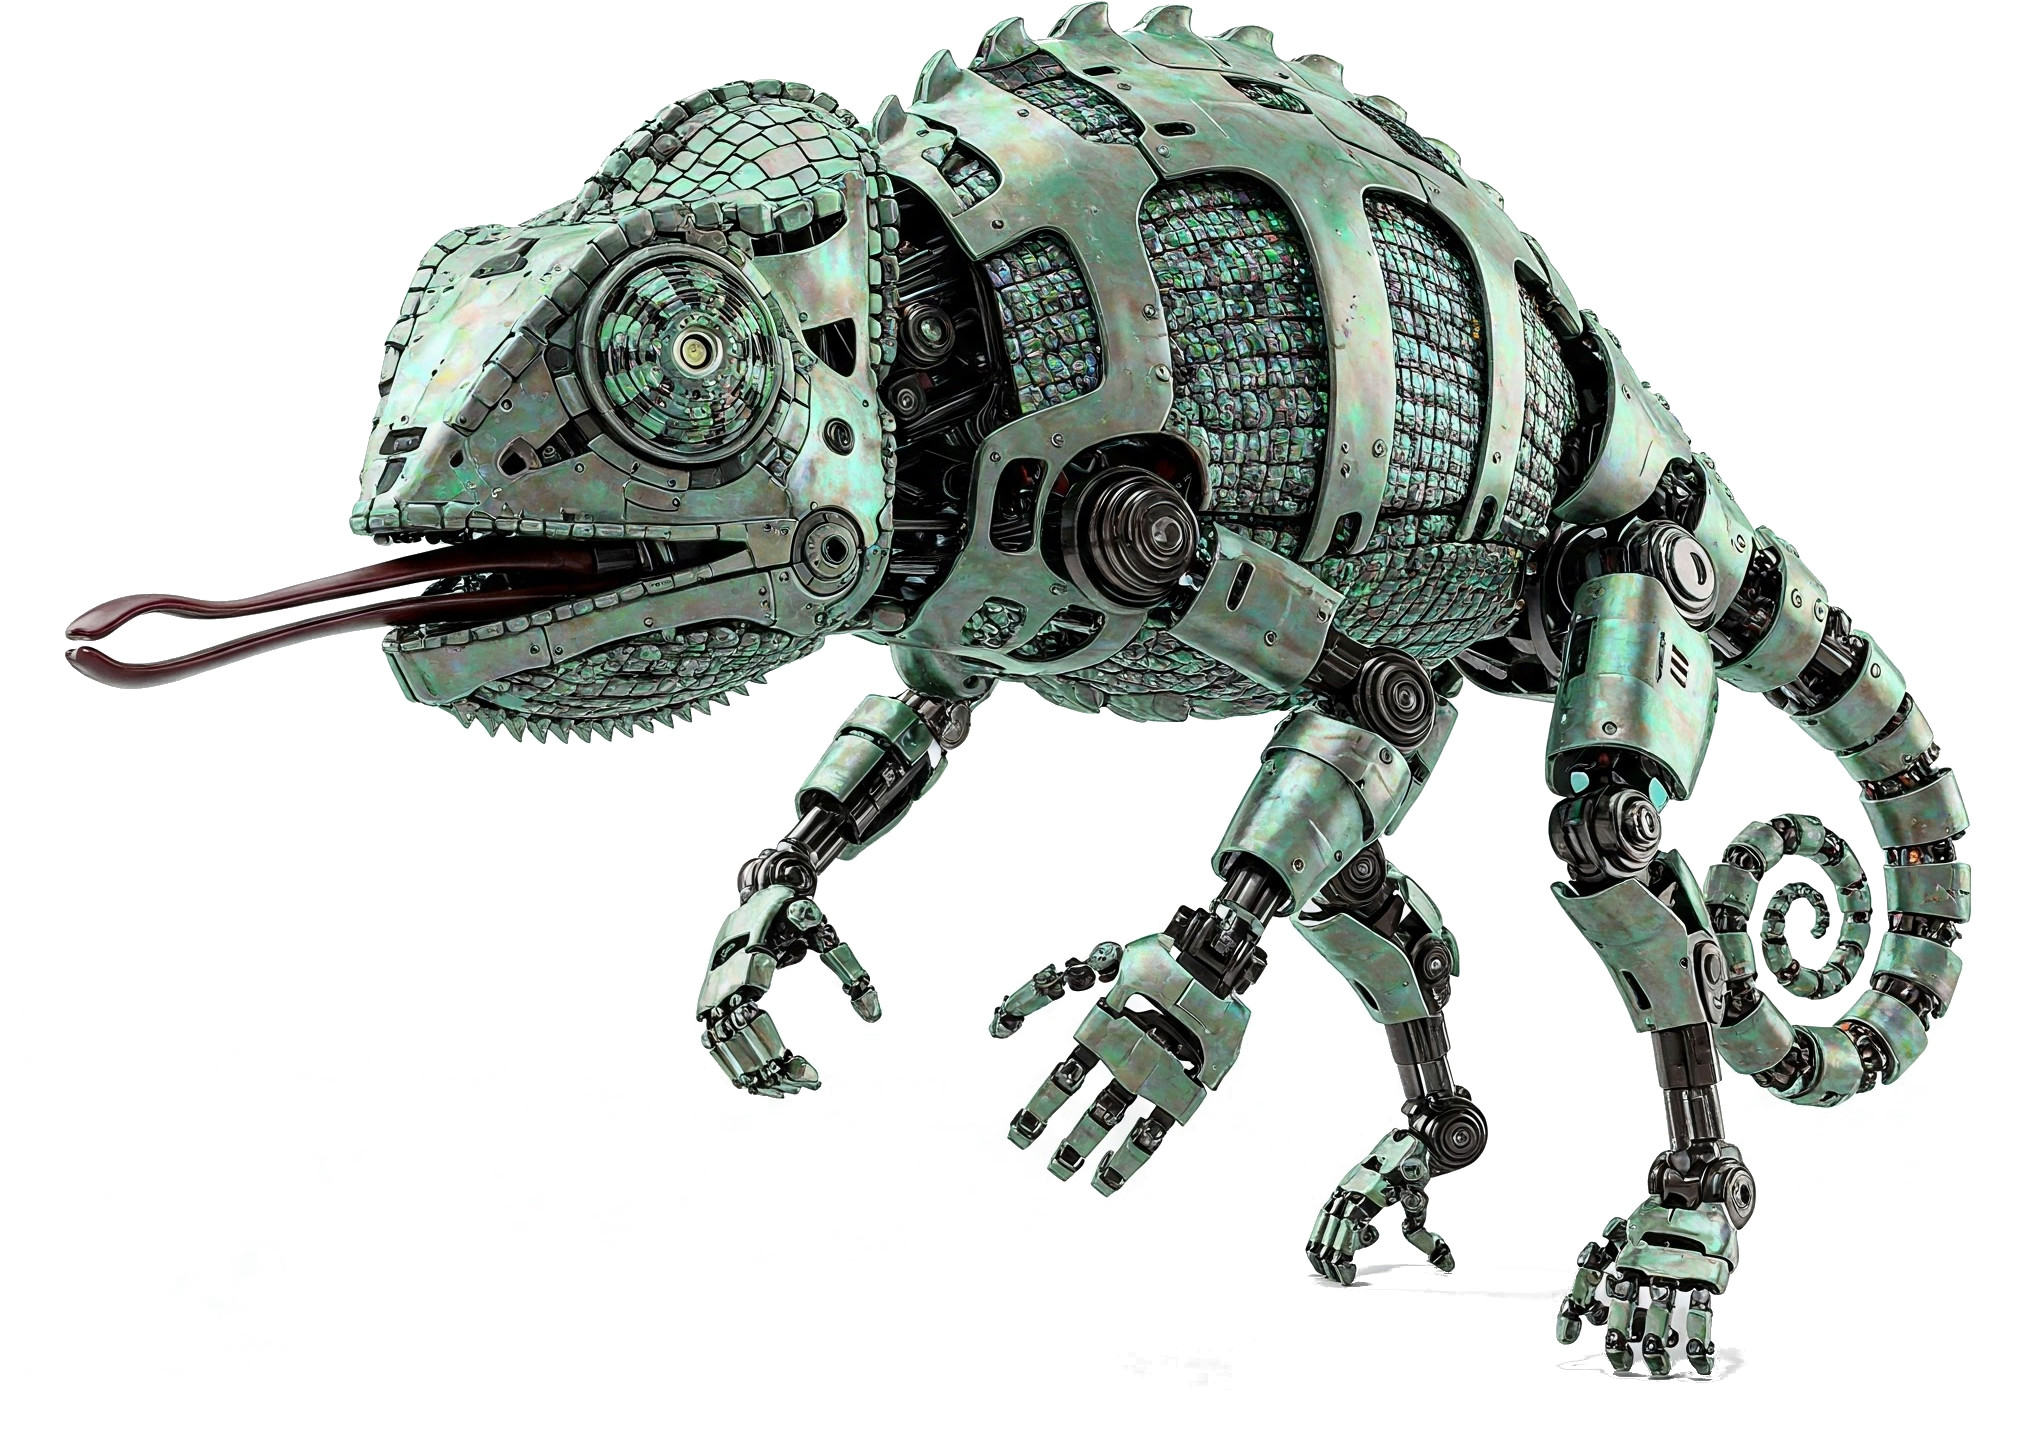
\includegraphics[width=\linewidth]{RobotChameleon}
\end{columns}
\end{frame}

\begin{frame}[fragile]{Example}
\begin{columns}
\column{0.5\textwidth}
\begin{itemize}
  \item Answers with standard prompt are extensive
  \item User has to select the right one
  \item Sensitive information may be shared!
\end{itemize}
\column{0.5\textwidth}
  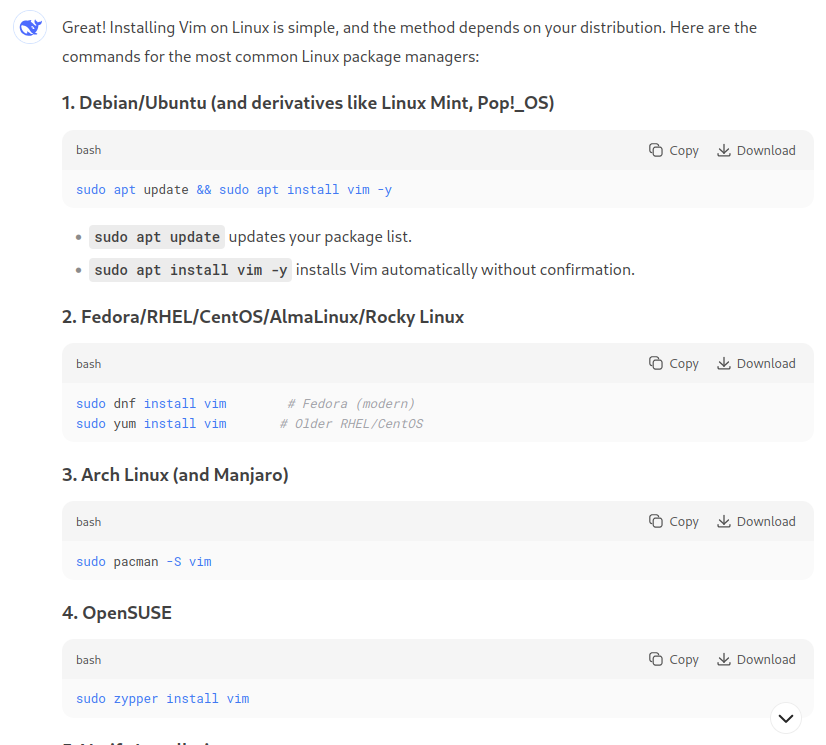
\includegraphics[width=\linewidth]{DeepSeek}
\end{columns}
\end{frame}

\begin{frame}[fragile]{Problem}
\begin{columns}
\column{.5\textwidth}
\begin{itemize}
  \item LLMs are created by training text completion on scraped sources
  \item LLMs don't have any context
\end{itemize}
\column{.5\textwidth}
  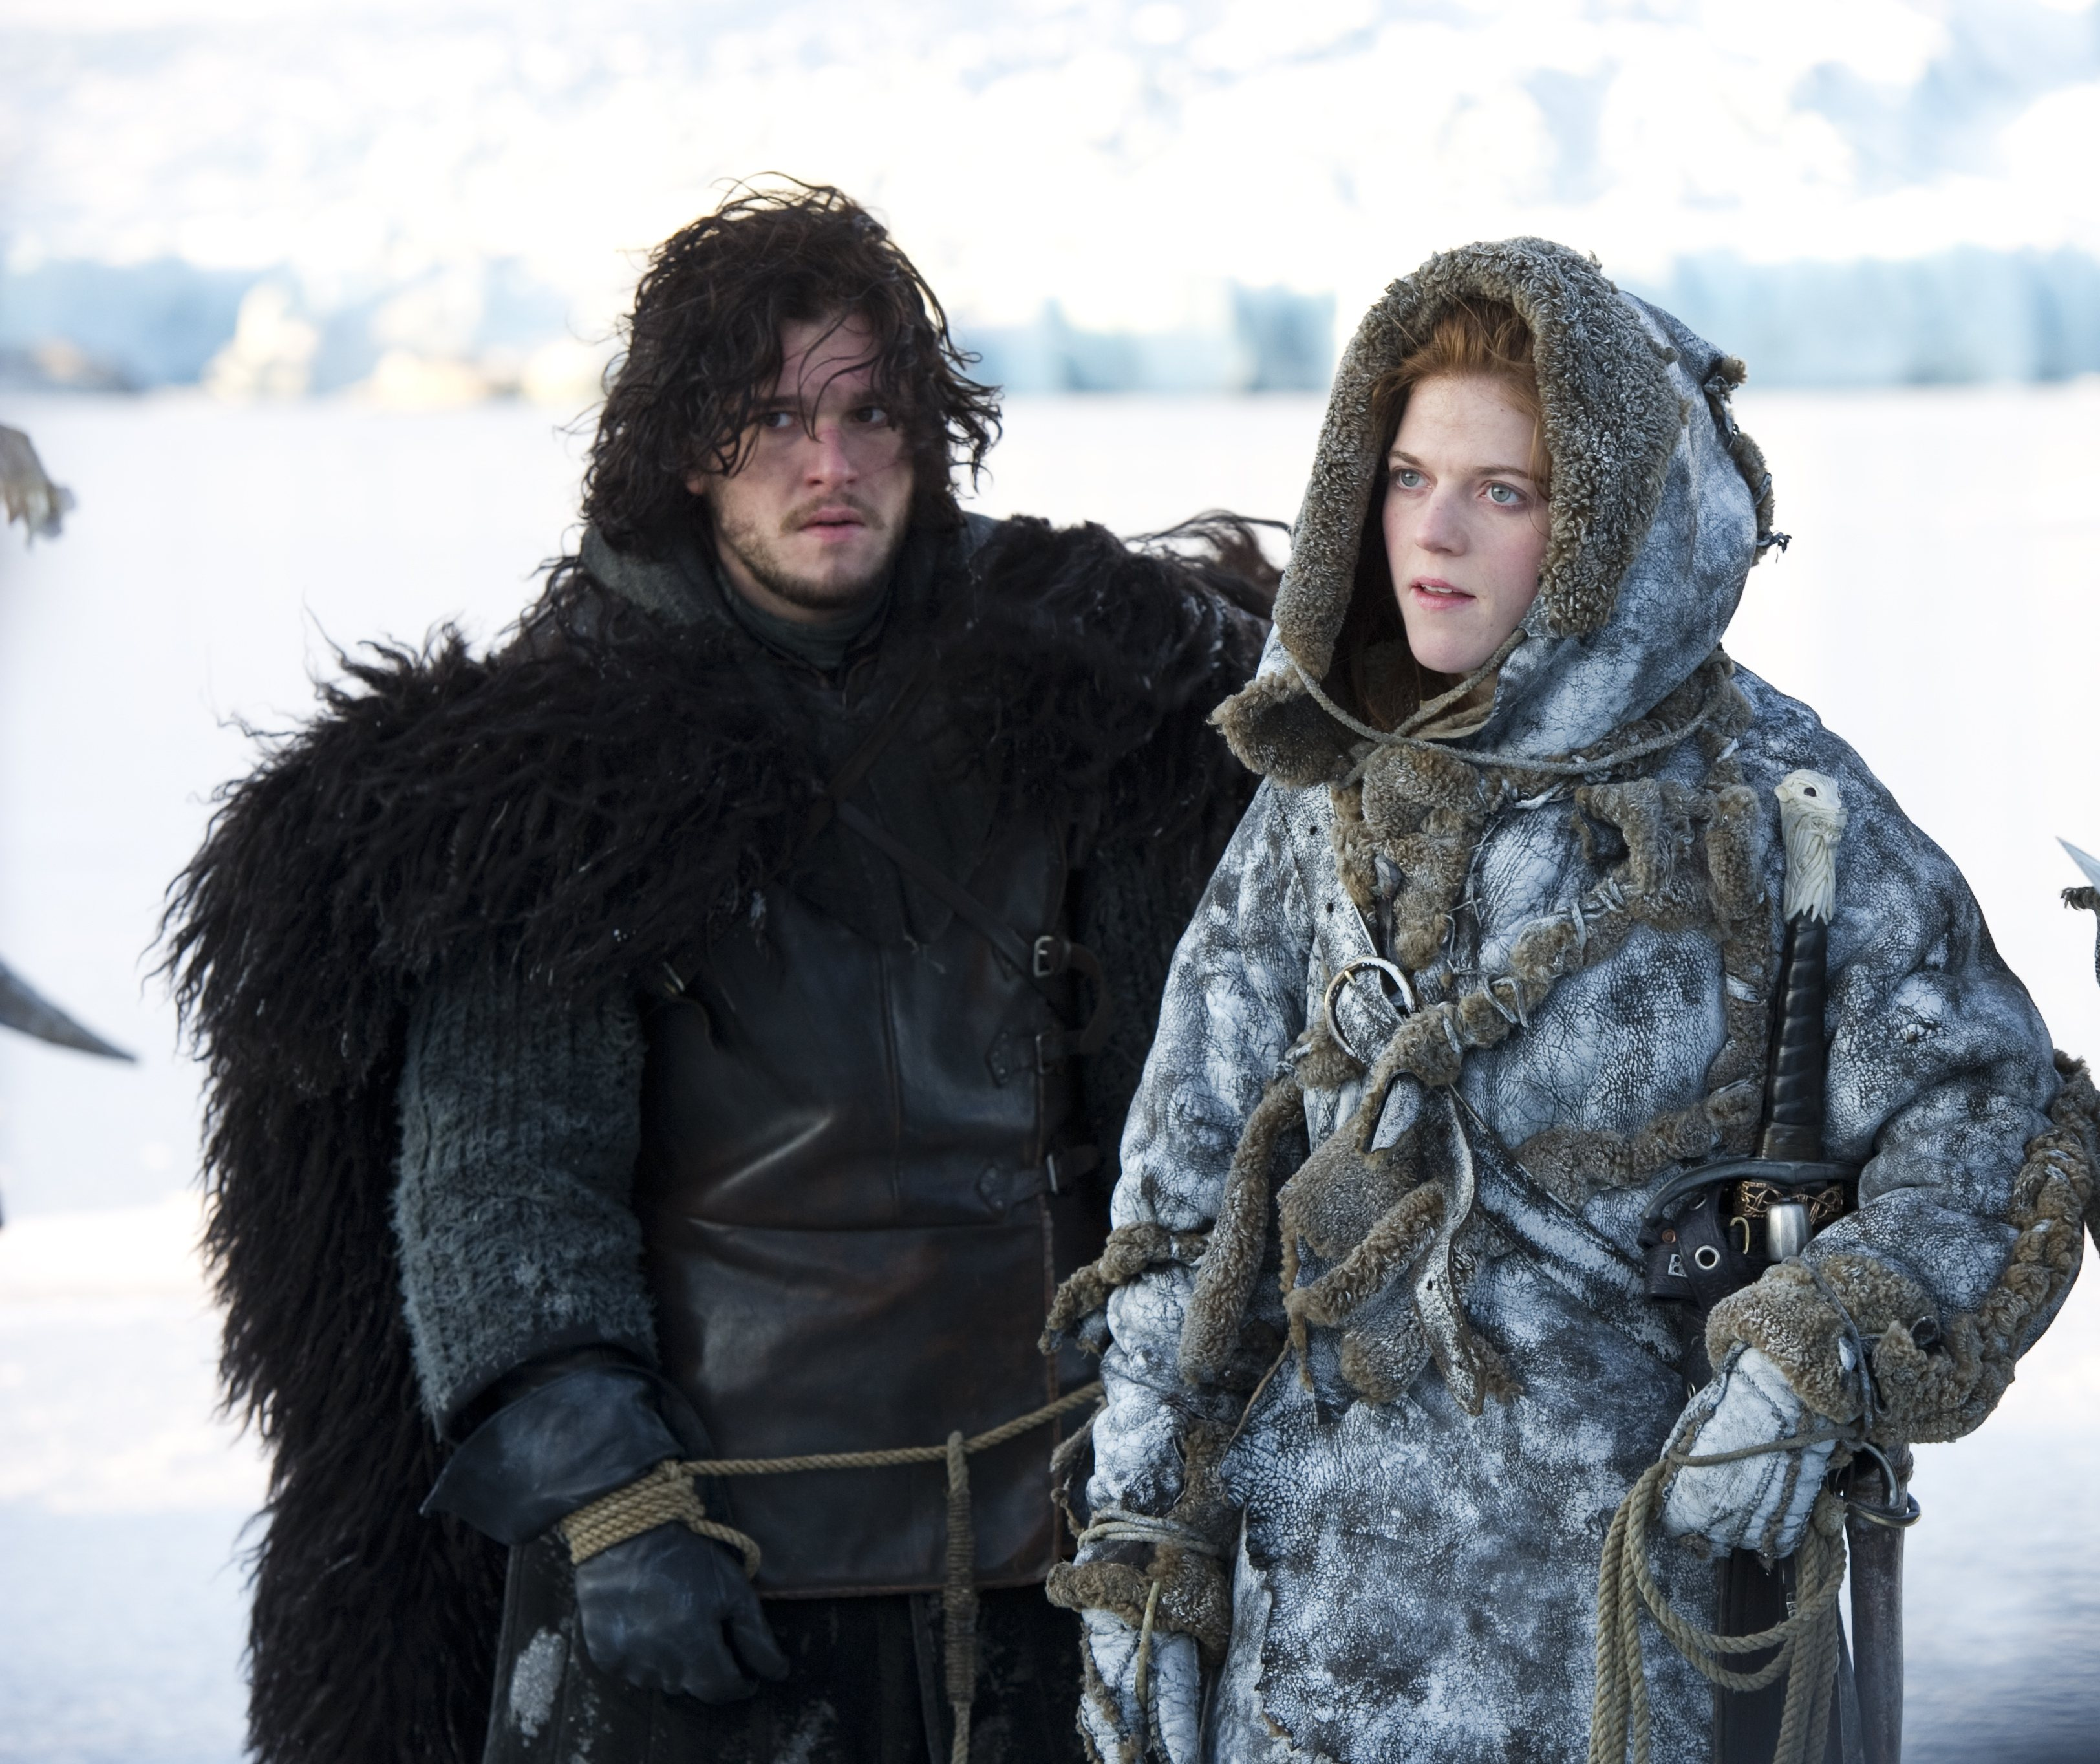
\includegraphics[width=\linewidth]{JohnSnow}
\textbf{You know nothing, John Snow!} 
\end{columns}
\end{frame}

\begin{frame}[fragile]{Solution}
\begin{columns}
\column{.5\textwidth}
\begin{itemize}
  \item Context is needed for accurate solutions
  \item Should be easy to get context of actual system.
\end{itemize}
\column{.3\textwidth}
  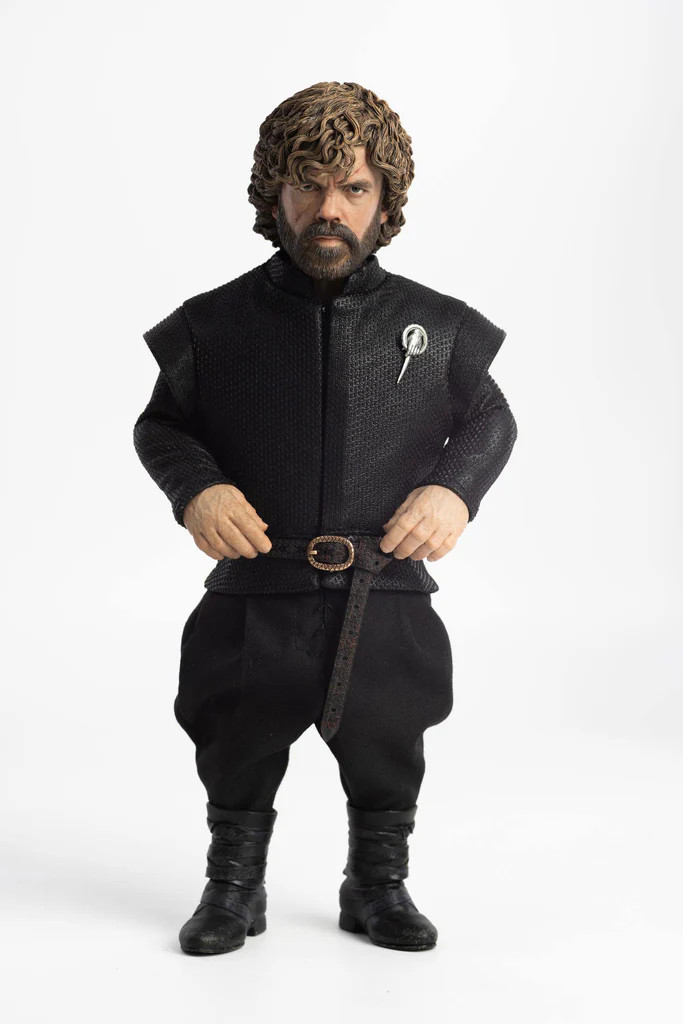
\includegraphics[width=\linewidth]{Tyrion}
\textbf{I know things!}
\end{columns}
\end{frame}

\begin{frame}{Introducing Kowalski: A Specialized AI Assistant}
\begin{columns}
\column{.5\textwidth}
  \begin{itemize}
    \item Kowalski is designed to bridge the gap between LLMs and system configuration.
    \item It provides LLMs with highly relevant and context-aware information.
    \item Focus on extracting and utilizing knowledge from technical documentation, specifically SUSE/SLE docs.
  \end{itemize}
\column{.3\textwidth}
  
\includegraphics[width=\linewidth]{Kowalski}
\end{columns}
\end{frame}

\section{AI Tools}
\begin{frame}{Vector Embeddings}
  \begin{block}{Definition}
  Numerical representations of data (words, texts, etc.) in a vector space
  \end{block}
  \begin{columns}
  \column{.7\textwidth}
  \begin{block}{Key Properties}
  \begin{itemize}
    \item Capture semantic relationships \\(e.g. "king" – "man" + "woman" ≈ "queen").
    \item Fixed-length
    \item Similar items cluster together in the vector space.
  \end{itemize}
  \end{block}
  \column{.3\textwidth}
  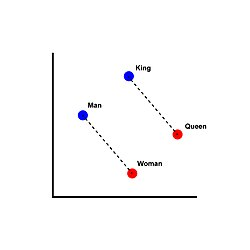
\includegraphics[width=\linewidth]{Word_vector_illustration}
  \end{columns}
  \begin{block}{Example}
  \texttt{"cat" → [0.2, -0.5, 0.7], "dog" → [0.3, -0.4, 0.6]}
  \end{block}
\end{frame}

\begin{frame}{Emedding details}
  \begin{block}{Creation methods}
  \begin{description}
    \item[GloVe]\hfill \\ Uses global word co-occurrence statistics from a corpus.
    \item[Word2Vec]\hfill \\predicts surrounding words (or target word) using shallow neural networks.
  \end{description}
  \end{block}
  \begin{block}{Vector space search}
  \begin{itemize}
    \item Searching nearest neighbors in high dimesional vector space isn't  trivial
    \item Facebook created \texttt{faiss} library which does this job
  \end{itemize}
  \end{block}
\end{frame}

\begin{frame}{Embedding conclusions}
\begin{columns}
\column{.5\textwidth}
\begin{itemize}
  \item Use \emph{Word2Vec} like embedding so that LLM and embedding run on Ollama
  \item Creation embedding for documentation is computational expensive
  \item Embeddings are available for with different OSS licenses, text lenghts and embedding dimenstions
\end{itemize}
\column{.5\textwidth}
  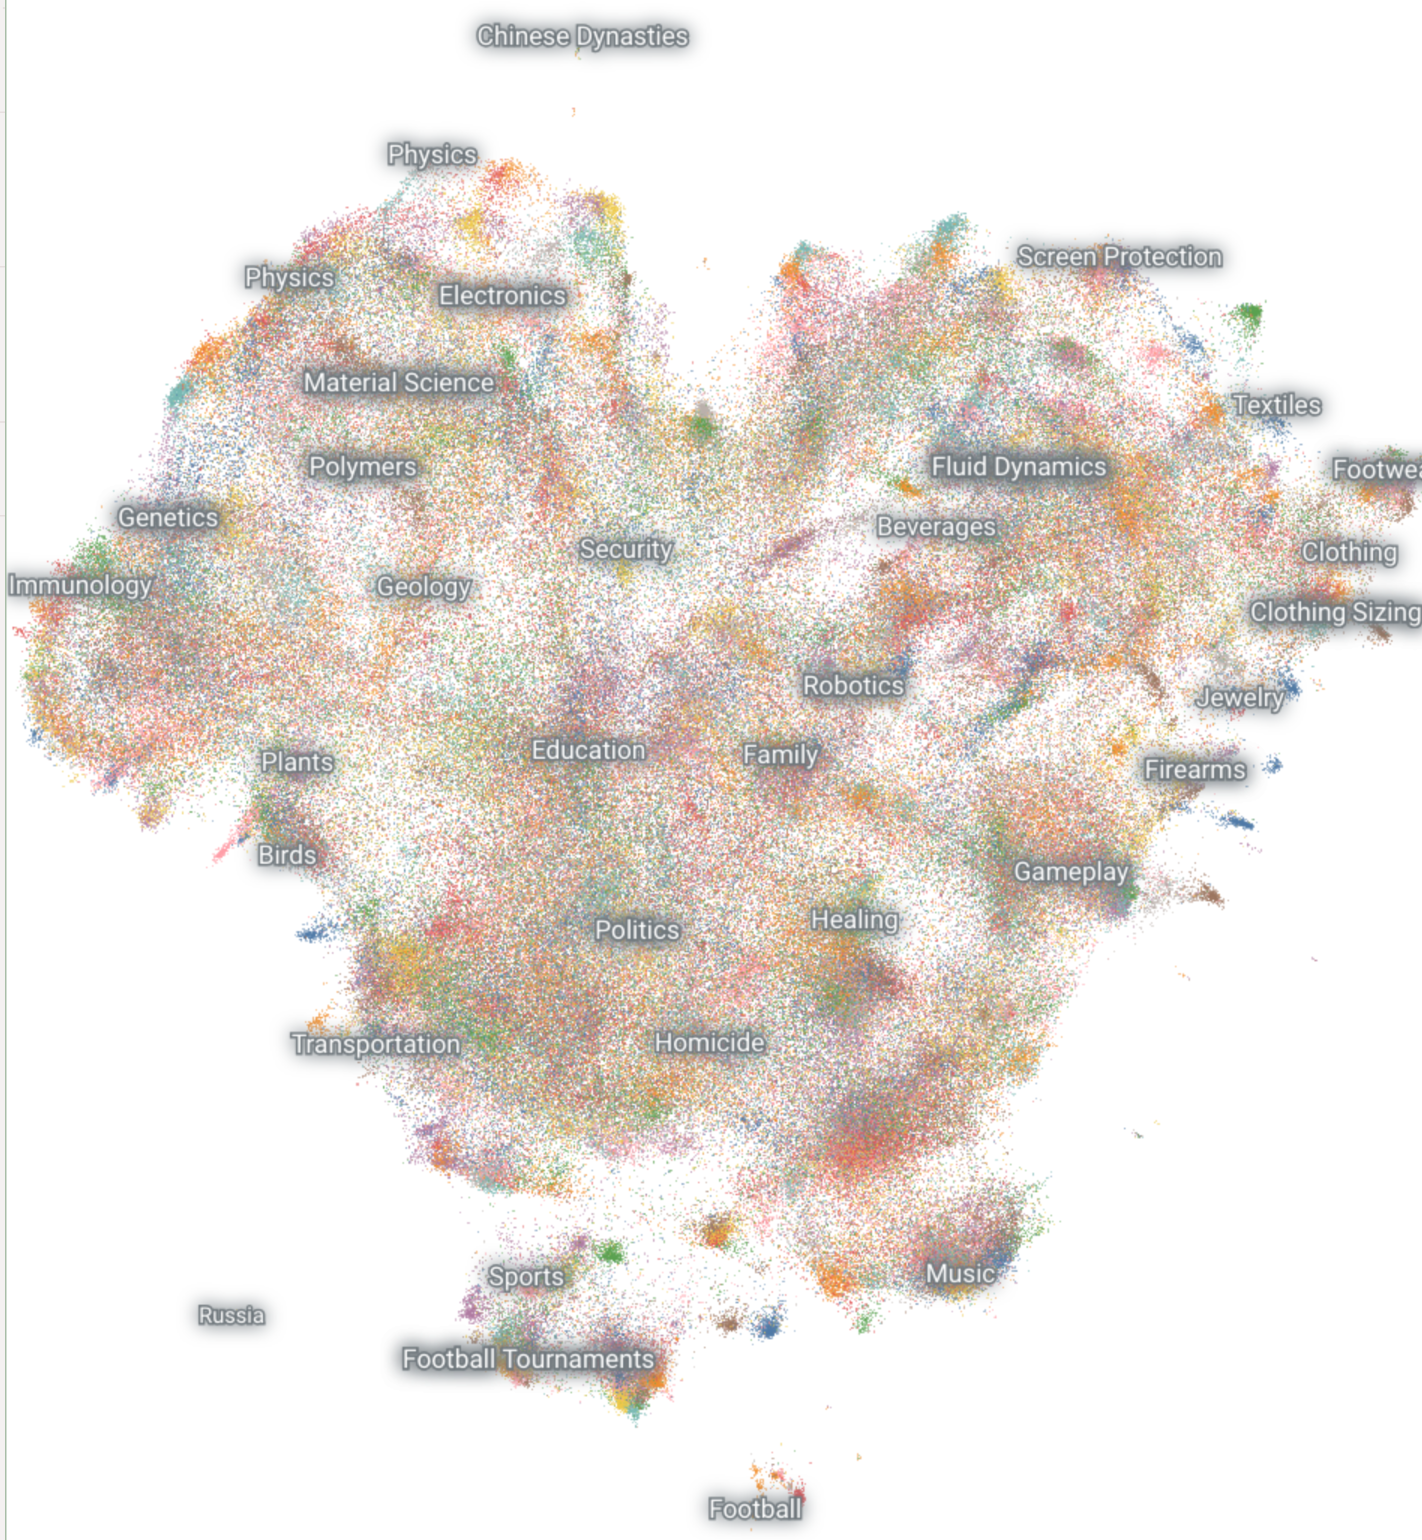
\includegraphics[width=\linewidth]{Noimic}
\end{columns}
\end{frame}


\begin{frame}{Ollama: Local AI Powerhouse}
\begin{itemize}
    \item Ollams is Open-source framework for running LLMs locally
    \item Enables execution of models like LLaMA on consumer hardware
\end{itemize}

\begin{block}{Efficiency}
\begin{itemize}
    \item Uses \textbf{quantization}—reduces model precision (e.g. 32-bit $\rightarrow$ 4-bit)
    \item Smaller model size + faster inference
    \item Minimal accuracy loss for significant performance gains
\end{itemize}
\end{block}

\begin{columns}
\column{.7\textwidth}
\begin{block}{The LLaMA Foundation}
\begin{itemize}
    \item Meta's LLaMA was first major open weights model
    \item Proved smaller models could compete with proper training
\end{itemize}
\end{block}
\column{.1\textwidth}

\includegraphics[width=\linewidth]{ollama.png}
\end{columns}
\end{frame}

\section{Kowalski Implementation}
\begin{frame}{Why Go for Kowalski?}
\begin{block}{Python's Challenges in Production AI}
\begin{itemize}
    \item \textbf{Dependency Hell}  
    \begin{itemize}
        \item Python has a \textit{long tail}—importing one package pulls in many others which have to packaged 
        \item Increases deployment complexity 
        \item e.g. python-faiss is not available for the \emph{oldest} python in Tumbleweed
    \end{itemize}
\end{itemize}
\end{block}

\begin{columns}
\column{.6\textwidth}
\begin{block}{Go's Advantages}
\begin{itemize}
    \item \textbf{Single Binary Deployment}  
    \begin{itemize}
        \item No dependency chains—statically linked executables  
    \end{itemize}
    \item \textbf{Compile Time Vendoring}  
    \begin{itemize}
        \item Dependencies are imported at copmile time and not run time 
    \end{itemize}
\end{itemize}
\end{block}
\column{.2\textwidth}

\includegraphics[width=\linewidth]{gopher}
\end{columns}
\end{frame}

\begin{frame}{How does Kowalski work}
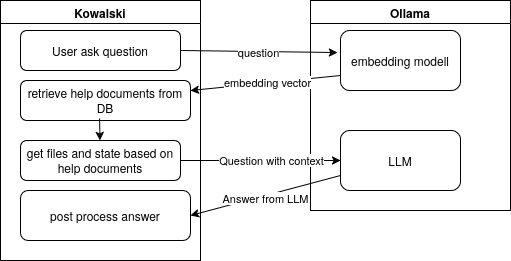
\includegraphics[width=\linewidth]{Flow.drawio}
\end{frame}

\end{document}
